\documentclass{article}
\author{Jim Lam}
\usepackage{hyperref}
\usepackage{amsmath}
\usepackage{amssymb}
\usepackage{tikz}
\usepackage{outlines}
\usetikzlibrary{automata, positioning, arrows}
\tikzset{
->, % makes the edges directed
node distance=3cm, % specifies the minimum distance between two nodes. Change if necessary.
every state/.style={thick, fill=gray!10}, % sets the properties for each ’state’ node
initial text=$ $, % sets the text that appears on the start arrow
}
\def\firstellip{(1.6, 0) ellipse [x radius=3cm, y radius=1.5cm, rotate=50]}
\def\secondellip{(0.3, 1cm) ellipse [x radius=3cm, y radius=1.5cm,
rotate=50]} \def\thirdellip{(-1.6, 0) ellipse [x radius=3cm, y radius=1.5cm,
rotate=-50]} \def\fourthellip{(-0.3, 1cm) ellipse [x radius=3cm, y
radius=1.5cm, rotate=-50]} \def\bounding{(-5,-3) rectangle (5,4)}
\def\exp{
    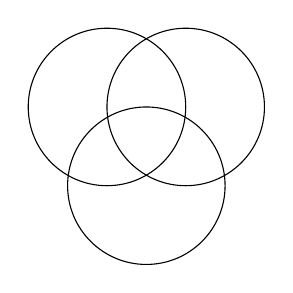
\begin{tikzpicture}
        %% You can adjust the opacity here. For venn diagrams it is convenient to have a low opacity so that you can see intersections
        \begin{scope} [fill opacity = .0]
            %% The draw command knows a lot of shapes. To make a rectangle you just need to specify two diagonal corners. Make sure you always have a semicolon at the end of your draw commands, otherwise latex flips out.
            %% Similarly, you can make a circle by specifying the center and then the radius. You can also add a fill color, but if you're printing in black and white you'll probably want to remove that line.
            \draw[fill=green, draw = black] (-0.5,1) circle (1);
            \draw[fill=blue, draw = black] (0.5,1) circle (1);
            \draw[fill=red, draw = black] (0,0) circle (1);
            %% We can use the node command to label points. If you put your cursor on "LARGE" or "textbf" a box will drop down with size and text style options.
            \node at (-0.9,1.4) {$\mathbf{A}$};
            \node at (0.9,1.4) {$\mathbf{B}$};
            \node at (0, -0.4) {$\mathbf{C}$};
        \end{scope}
        %% And now you have a venn diagram. Yay!
        %\draw[help lines](-5,5) grid (5,-6);    This line can draw the grid lines to help guide you. I use these when I'm writing the code and then delete this line when I publish the pdf.
    \end{tikzpicture}
}
\begin{document}
\title{%
    COM1026 EXAM NOTES, CONDENSED \\
    \large 01 IFH 02 - Ada \\
    Lovelace Lab 129 \\
    Time: 15:30 - 17:30 \\
    }
\maketitle
\tableofcontents
\section{Set Theory}

\subsection{Introduction}
Quick recap on Naive set theory, meaning:

1. Introducing the basic concept of sets;

2. Introduce notation;

3. Illustrate Union, Intersection, and Set Difference operations;

4. Venn diagrams as proof;

5. Power sets;

6. How to proof with more rigor.

\subsection{Set Definition}

Question: Why are sets relevant to computing?

We have to represent data to compute it.
To group data, we put it into sets.

Some sets that I have seen before:
\begin{align*}
    \text{The set of natural numbers: } \mathbb{N} & = \{1, 2, 3, ...\}                    \\
    \text{The set of integers: } \mathbb{Z}        & = \{..., -3, -2, -1, 0, 1, 2, 3,...\}
\end{align*}
Question: What are sets?

% generate a heavily stylised latex quote of the definition of a set below.

A set is a collection of objects, called elements of the set. The elements of a set can be anything, but they must be distinct.

\subsection{Notation}
Sets are denoted with capital letters, e.g. A, B, C. The elements of a set are listed inside curly brackets:
\begin{align*}
    A & = \{1, 2, 3\}                \\
    B & = \{a, b, c, d, e, f, g, h\}
\end{align*}

\subsubsection{Cardinality}

The cardinality of a set is the number of elements in the set. The cardinality of a set is denoted with vertical bars, with the hash, or alternatively, the function $card$:
\begin{align*}
    \text{Card}(A)  & = |A| = 3 \\
    \#\{1,2,3,4,5\} & = 5       \\
    \#A             & = 3       \\  % hash also works.
    \#\mathbb{N}    & = \infty
\end{align*}
\subsubsection{Abstraction axiom}
GIven a property $P(x)$, we can define a set $A$ as:
\begin{align*}
    A & = \{x | P(x)\}
\end{align*}
In other words, whatever property P, there exists a set A containing the objects that satisfy P and only these objects.

\subsubsection{Set builder notation}
Other than enumerating the elements of a set, there are other ways to describe a set. Verbal descriptions and adding an inclusion rule to the set builder notation are two more examples:
\begin{align*}
    C & = \{x | x \in \mathbb{N}, 0 \leq x \leq 5\}                    \\
      & = \{x |\text{$x$ is in the appropriate set}, 0 \leq x \leq 5\}
\end{align*}

\subsubsection{Empty set}
The empty set is a set with no elements. It is denoted $\emptyset$ or $\{\}$.
\begin{align*}
    \emptyset & = \{\}               \\
    \emptyset & \neq \{ \emptyset \}
\end{align*}

\subsection{Basic set operations}
\subsubsection{Membership}
The membership relation is denoted $\in$ and is used to indicate that an element is in a set.
Conversely, $\notin$ is used to indicate that an element is not in a set.
\begin{align*}
    \text{Let the set } A & = \{1, 2, 3\}  \\
    1 \in A               & = \text{True}  \\
    3 \notin A            & = \text{False} \\
\end{align*}
To denote a subset, we use $\subseteq$.
Since a subset can include the set itself, we use $\subset$ to denote a proper subset.
\begin{align*}
    \text{Let the set } A & = \{1, 2, 3\}  \\
    \{1, 2\} \subseteq A  & = \text{True}  \\
    \{1, 2, 3\} \subset A & = \text{False} \\
\end{align*}

\subsubsection{Union, intersection, and set difference}

The union of two sets A and B is denoted $A \cup B$ and contains all elements of both sets.

The intersection $A \cap B$ contains elements common to both.

Set diffrence $A \setminus B$ contains elements in A but not in B. (Note: A must come first, otherwise the result is different.)
\begin{align*}
    A \cup B      & = \{1, 2, 3, a, b, c\} \\
    A \cap B      & = \{1, 2, 3\}          \\
    A \setminus B & = \{1, 2, 3\}          \\
\end{align*}

\subsection{Venn diagrams}
Venn diagrams are a way to visualise sets and their operations.
Use circles to represent sets, and shading to distinguish areas of interest.

\begin{align*}
    \text{Let the set } = \{1, 2, 3\} \\
    \text{Let the set } = \{2, 3, 4\} \\
    \text{Let the set } = \{3, 4, 5\} \\
    (C \cup B) \cap A = \{4, 5\}      \\
    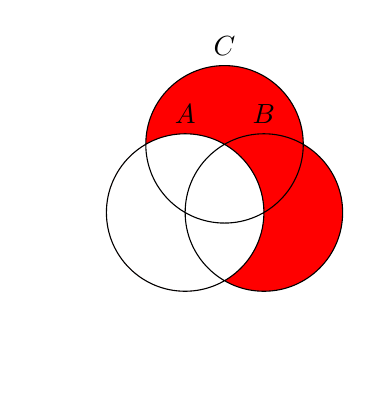
\begin{tikzpicture}[fill=red]
        % left hand
        \scope
        \clip (-2,-2) rectangle (2,2)
        (0,0) circle (1);
        \fill (0,0) circle (1);
        \endscope
        % right hand
        \scope
        \clip (-2,-2) rectangle (2,2)
        (0,0) circle (1);
        \fill (1,0) circle (1);
        \endscope
        \scope
        \clip (-2,-2) rectangle (2,2)
        (0,0) circle (1);
        \fill (0.5,0.866) circle (1);
        \endscope
        % outline
        \draw (0,0) circle (1) (0,1)  node [text=black,above] {$A$}
        (1,0) circle (1) (1,1)  node [text=black,above] {$B$}
        (0.5,0.866) circle (1) (0.5,1.866)  node [text=black,above] {$C$};
    \end{tikzpicture}
\end{align*}

% \subsubsection{Template for a venn diagrams:}

% \begin{align*}
%     \exp
% \end{align*}

\pagebreak

Here is a more complicated example involving 4 sets:

Refrenced from \url{https://www.overleaf.com/latex/examples/example-venn-diagram-with-isolated-areas-filled/xjptmqsjfdlc}

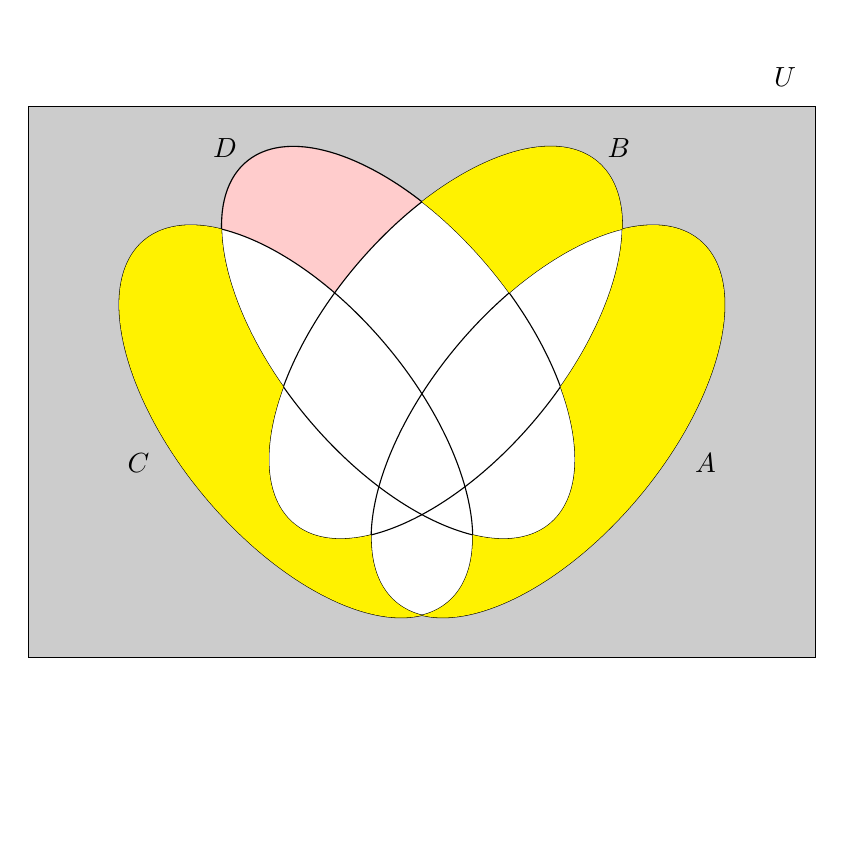
\begin{tikzpicture} \filldraw[fill=black, opacity=0.2] \bounding;

    \scope \fill[white] \fourthellip; \endscope \filldraw[fill=red,
        opacity=0.2] \fourthellip;

    %single colors
    \scope \fill[white] \secondellip; \fill[white] \thirdellip; \fill[white]
    \firstellip; \endscope

    \draw \firstellip node [label={[xshift=2.0cm, yshift=-0.9cm]$A$}] {};
    \draw \secondellip node [label={[xshift=2.2cm, yshift=2.1cm]$B$}] {};
    \draw \thirdellip node [label={[xshift=-2.0cm, yshift=-0.9cm]$C$}] {};
    \draw \fourthellip node [label={[xshift=-2.2cm, yshift=2.1cm]$D$}] {};
    \draw \bounding node [label=above left:$U$] {};

    \begin{scope}
        \begin{scope}[even odd rule]% first ellipse corner
            \clip \secondellip (-5,-5) rectangle (5,5);
            \clip \thirdellip (-5,-5) rectangle (5,5);
            \clip \fourthellip (-5,-5) rectangle (5,5);
            \fill[yellow] \firstellip;
        \end{scope}
    \end{scope}

    \begin{scope}
        \begin{scope}[even odd rule]% second ellipse corner
            \clip \firstellip (-5,-5) rectangle (5,5);
            \clip \thirdellip (-5,-5) rectangle (5,5);
            \clip \fourthellip (-5,-5) rectangle (5,5);
            \fill[yellow] \secondellip;
        \end{scope}
    \end{scope}

    \begin{scope}
        \begin{scope}[even odd rule]% third ellipse corner
            \clip \secondellip (-5,-5) rectangle (5,5);
            \clip \firstellip (-5,-5) rectangle (5,5);
            \clip \fourthellip (-5,-5) rectangle (5,5);
            \fill[yellow] \thirdellip;
        \end{scope}
    \end{scope}

\end{tikzpicture}

This covers the basics of set notation and operations.

\pagebreak

\subsection{Power sets}

The power set of a set is the set of all subsets of that set.

The power set of a set A is denoted in various ways, including $2^A$, $\mathcal{P}(A)$, $\mathbb{P}(A)$, or $\wp(A)$.

\begin{align*}
    \text{Let the set } A                 & = \{1, 2, 3\}                                                                   \\
    \wp(A)                                & = \{\emptyset, \{1\}, \{2\}, \{3\}, \{1, 2\}, \{1, 3\}, \{2, 3\}, \{1, 2, 3\}\} \\
    \text{More generally: } \mathbb{P}(A) & = \{B | B \subseteq A\}
\end{align*}

\subsection{Proofs}

\subsubsection{Proof by property}

Proposition (example from lecutre notes): For any sets A, B, and C:

\begin{align*}
    A\setminus (B\cup C) = (A\setminus B)\cap (A\setminus C)
\end{align*}

Recapping some of the basic properties of sets, using sets S and T, and element x:

\begin{align*}
     & \text{Property 1: } & S \subseteq T \text{ and } T \subseteq S  & \iff S = T               \\
     & \text{Property 2: } & (\text{For any x} \in S \implies x \in T) & \iff S \subseteq T       \\
     & \text{Property 3: } & x \in S \text{ and } x \in T              & \iff x \in S \cap T      \\
     & \text{Property 4: } & x \in S \text{ or } x \in T               & \iff x \in S \cup T      \\
     & \text{Property 5: } & x \in S \text{ and } x \notin T           & \iff x \in S \setminus T \\
     & \text{Property 6: } & x \notin S \text{ and } x \notin T        & \iff x \notin T \cup S   \\
\end{align*}

Using property 1, we can prove that two sets are equal by proving that each is a subset of the other.

\begin{align*}
     & \text{Let } x \in A\setminus (B\cup C)                                      \\
     & \iff x \in A \text{ and } x \notin B \cup C                                 \\
     & \iff x \in A \text{ and } x \notin B \text{ and } x \notin C                \\
     & \iff x \in A \setminus B \text{ and } x \in A \setminus C                   \\
     & \iff x \in (A \setminus B) \cap (A \setminus C)                             \\
     & \therefore A\setminus (B\cup C) \subseteq (A\setminus B)\cap (A\setminus C) \\
\end{align*}

Doing this for the other direction:

\begin{align*}
     & A\setminus (B\cup C)= (A\setminus B)\cap (A\setminus C)                           \\
     & \text{Let } x\in (A\setminus B)\cap (A\setminus C)                                \\
     & \iff x \in A\setminus B \text{ and } x \in A\setminus C                           \\
     & \iff x \in A \text{ and } x \notin B \text{ and } x \in A \text{ and } x \notin C \\
     & \iff x \in A \text{ and } x \notin B \cup C                                       \\
     & \iff x \in A \setminus (B \cup C)                                                 \\
     & \therefore (A\setminus B)\cap (A\setminus C) \subseteq A\setminus (B\cup C)
\end{align*}

\subsection{Von Neumann Ordinals}

The von Neumann ordinals are a way of representing the natural numbers using sets.


% let 0 = ∅
% let • 𝑛 + 1 = 𝑛 ∪ {𝑛}
let $0 = \emptyset$, $n + 1 = n \cup \{n\}$:

\begin{align*}
    0 & = \emptyset                                                                \\
    1 & = \{0\} = \{\emptyset\}                                                    \\
    2 & = \{0, 1\} = \{\emptyset, \{\emptyset\}\}                                  \\
    3 & = \{0, 1, 2\} = \{\emptyset, \{\emptyset\}, \{\emptyset, \{\emptyset\}\}\} \\
    n & = \{0, 1, 2, ..., n-1\} \text{ you get the idea}
\end{align*}

\section{Relations}

\subsection{Cartesian product and relations}

The cartesian product of two sets A and B is the set of all ordered pairs (x, y), where: $x \in A$ and $y \in B$.
The cartesian product of A and B is denoted as $A \times B$.

Example:

\begin{align*}
    Books               & = \{1984, \text{Concrete}, \text{Incerto}\}                                                                    \\
    Rating              & = \{\text{Good}, \text{Evil}, \text{Unimportant}\}                                                             \\
    Books \times Rating & = \{(1984, \text{Good}), (1984, \text{Evil}), (1984, \text{Unimportant})\}                                     \\
                        & \cup \{(\text{Concrete}, \text{Good}), (\text{Concrete}, \text{Evil}), (\text{Concrete}, \text{Unimportant})\} \\
                        & \cup \{(\text{Incerto}, \text{Good}), (\text{Incerto}, \text{Evil}), (\text{Incerto}, \text{Unimportant})\}
\end{align*}

A relation R from A to B is a subset of the cartesian product of A and B. i.e. $R \subseteq A \times B$.
Taking the example above, we can define a relation R from Books to Rating as:

\begin{align*}
    R = \{(1984, \text{Good}), (\text{Concrete}, \text{Evil}), (\text{Incerto}, \text{Unimportant})\}
\end{align*}

Note that R is a subset of the cartesian product of Books and Rating.

\subsection{Relation notation}

There are three main ways to denote a relation R from A to B:

\begin{itemize}
    \item Ordered pairs
    \item Table
    \item Mapping
\end{itemize}

Should you want to confuse yourself even further, the infix notation is a good option.

\begin{align*}
     & \text{Let the relation "likes" be defined as: } \mathbf{L} = \{(x, y) | x \text{ likes } y\} \\
     & \text{You can denote (x, y) as a member of the likes by writing: x$\mathbf{L}$y}             \\
\end{align*}

\subsection{Representing relations}

Since winter is approaching, let's define a relation "likes" from people to clothing.

\begin{align*}
    \text{Let the set of people } P     & = \{\text{Jim}, \text{Bob}, \text{Alice}, \text{Eve}, \text{Mallory}\}     \\
    \text{Let the set of clothing } C   & = \{\text{Jacket}, \text{Scarf}, \text{Gloves}, \text{Hat}, \text{Socks}\} \\
    \text{Let the relation } \mathbf{L} & = \{(x, y) | x \text{ likes } y\}                                          \\
    \text{In table form:}                                                                                            \\
    \begin{tabular}{|l|l|l|l|l|l|l|}
        \hline
        P       & L      \\
        \hline
        Jim     & Scarf  \\
        \hline
        Bob     & Jacket \\
        \hline
        Alice   & Scarf  \\
        \hline
        Eve     & Gloves \\
        \hline
        Mallory & Hat    \\
        \hline
        Mallory & Socks  \\
        \hline
    \end{tabular}
\end{align*}

Since a table popped into your view, it is as good a time as any to introduce it's application in databases.

Given this example relation of students and their various attributes, we can represent it in a table.

\begin{align*}
    \text{Let the set of students } S   = \{\text{Jim}, \text{Bob}, \text{Alice}, \text{Eve}, \text{Mallory}\}                         \\
    \text{Let the set of attributes } A = \{\text{name}, \text{Age}, \text{Height}, \text{Weight}, text{Happiness}, \text{Net Worth}\} \\
    \text{Let the relation } \mathbf{R} = \{(x, y) | x \text{ has attribute } y\}                                                      \\
    \text{In table form:}                                                                                                              \\
    \begin{tabular}{|l|l|l|l|l|l|l|}
        \hline
        Name    & Age & Height & Weight & Happiness & Net Worth \\
        \hline
        Jim     & 20  & 180    & 80     & 0.5       & 0.1       \\
        \hline
        Bob     & 21  & 170    & 70     & 0.6       & 0.2       \\
        \hline
        Alice   & 19  & 160    & 60     & 0.7       & 0.3       \\
        \hline
        Eve     & 18  & 150    & 50     & 0.8       & 0.4       \\
        \hline
        Mallory & 17  & 140    & 40     & 0.9       & 0.5       \\
        \hline
    \end{tabular}
\end{align*}

We can extract information by getting a subset of relations.

For example: $(\text{Jim}, \text{180}) \in \text{Height}$

\subsection{Domain and range}

The domain of a relation is the set of all first elements of the ordered pairs in the relation.

\begin{align*}
    Dom(\mathbf{L}) & = \{x \in A \mid \exists x \in A : (x, y) \in \mathbf{L}\}
\end{align*}

The range of a relation is the set of all second elements of the ordered pairs in the relation.

\begin{align*}
    Ran(\mathbf{L}) & = \{y \in B \mid \exists y \in B : (x, y) \in \mathbf{L}\}
\end{align*}

\subsection{Relational composition}

The relational composition of two relations $\mathbf{R}$ and $\mathbf{S}$ is the relation $\mathbf{R} \circ \mathbf{S}$ (or $\mathbf{R};\mathbf{S}$, used to avoid confusion with function composition) defined as:

\begin{align*}
    \mathbf{R} ; \mathbf{S} & = \{(x, z) \mid \exists y \in B : (x, y) \in \mathbf{R} \text{ and } (y, z) \in \mathbf{S}\} \\
    \text{EXAMPLE:}                                                                                                        \\
    \mathbf{R}              & = \{(1, 2), (2, 3), (3, 4)\}                                                                 \\
    \mathbf{S}              & = \{(2, 3), (3, 4), (4, 5)\}                                                                 \\
    \mathbf{R} ; \mathbf{S} & = \{(1, 3), (2, 4), (3, 5)\}
\end{align*}

\subsection{Closures and equivalence classes}

\subsubsection{Property of relations}

A relation $\mathbf{R}$ is reflexive if $\forall x \in A : (x, x) \in \mathbf{R}$.

A relation $\mathbf{R}$ is symmetric if $\forall x, y \in A : (x, y) \in \mathbf{R} \implies (y, x) \in \mathbf{R}$.

A relation $\mathbf{R}$ is transitive if $\forall x, y, z \in A : (x, y) \in \mathbf{R} \text{ and } (y, z) \in \mathbf{R} \implies (x, z) \in \mathbf{R}$.



\subsubsection{Closures}

The closure of a relation $\mathbf{R}$ is the smallest relation containing $\mathbf{R}$ that is transitive.

Example of constructing a reflexive closure:

\begin{align*}
    \text{Let the relation } \mathbf{R}         & = \{(1, 2), (2, 3), (3, 4)\}                                 \\
    \text{The reflexive closure of } \mathbf{R} & = \{(1, 1), (1, 2), (2, 3), (3, 4), (2, 2), (3, 3), (4, 4)\}
\end{align*}

Example of constructing a symmetric closure:

\begin{align*}
    \text{Let the relation } \mathbf{R}         & = \{(1, 2), (2, 3), (3, 4)\}                         \\
    \text{The symmetric closure of } \mathbf{R} & = \{(1, 2), (2, 3), (3, 4), (2, 1), (3, 2), (4, 3)\}
\end{align*}

Example of constructing a transitive closure:

\begin{align*}
    \text{Let the relation } \mathbf{R}          & = \{(1, 2), (2, 3), (3, 4)\}                         \\
    \text{The transitive closure of } \mathbf{R} & = \{(1, 2), (2, 3), (3, 4), (1, 3), (2, 4), (1, 4)\}
\end{align*}


\subsubsection{Equivalence classes}

let $\rho \subseteq A \times A$ be an equivalence relation on A, given $A \neq \emptyset$, $a \in A$ be an arbitrary element of A.

NOTE: MUST CONSTRUCT EQUIVALENCE RELATION BEFORE CONSTRUCTING EQUIVALENCE CLASSES.

\begin{align*}
    [a]_{\rho} & = \{x \in A \mid (a, x) \in \rho\}
\end{align*}

\subsubsection{More properties of relations}

\begin{itemize}
    \item A relation $\mathbf{R}$ is antisymmetric if $\forall x, y \in A : (x, y) \in \mathbf{R} \text{ and } (y, x) \in \mathbf{R} \implies x = y$.
    \item A relation $\mathbf{R}$ is a partial order if it is reflexive, antisymmetric, and transitive.
    \item A connex relation is a relation $\mathbf{R}$ such that $\forall x, y \in A : (x, y) \in \mathbf{R} \text{ or } (y, x) \in \mathbf{R}$.
    \item Total order means that a relation is a partial order and a connex relation.
\end{itemize}
\section{Functions}

\subsection{Definition}

What is a function in the context of discrete mathematics?

A function is a relation $\mathbf{f}$ from A to B such that every element in A is mapped to exactly one element in B, i.e.:

$\forall x \in A . \forall y, z \in B : ((x, y) \in {f} \land (x, z) \in {f} \implies y = z)$.

\subsection{Notation}

A function $\mathbf{f}$ from A to B is denoted as $\mathbf{f} : A \rightarrow B$.

\subsection{Injective, surjective, bijective}

\begin{itemize}
    \item A function $\mathbf{f} : A \rightarrow B$ is injective if $\forall x, y \in A : \mathbf{f}(x) = \mathbf{f}(y) \implies x = y$.
    \item A function $\mathbf{f} : A \rightarrow B$ is surjective if $\forall y \in B : \exists x \in A : \mathbf{f}(x) = y$.
    \item A function $\mathbf{f} : A \rightarrow B$ is bijective if it is both injective and surjective.
\end{itemize}

\subsection{Composition}

The composition of two functions $\mathbf{f} : A \rightarrow B$ and $\mathbf{g} : B \rightarrow C$ is the function $\mathbf{g} \circ \mathbf{f} : A \rightarrow C$ defined as:

\begin{align*}
    \mathbf{g} \circ \mathbf{f} & = \{(x, z) \mid \exists y \in B : (x, y) \in \mathbf{f} \text{ and } (y, z) \in \mathbf{g}\}
\end{align*}

\subsection{Inverse}

The inverse of a function $\mathbf{f} : A \rightarrow B$ is the function $\mathbf{f}^{-1} : B \rightarrow A$ defined as:

\begin{align*}
    \mathbf{f}^{-1} & = \{(y, x) \mid (x, y) \in \mathbf{f}\}
\end{align*}

\section{Language and regular expressions}

\subsection{Alphabet}

We specify an Alphabet using the symbol $\Sigma$.

Examples:

\begin{align*}
    \Sigma_1 & = \{a, b, c, d, e, f\}                                                                                             \\
    \Sigma_2 & = \{0, 1, 2, 3, 4, 5, 6, 7, 8, 9\}                                                                                 \\
    \Sigma_3 & = \{S \mid S \subseteq \Sigma_1\}                     & (\text{The power set of } \Sigma_1, \#\Sigma_3 = 2^6 = 64) \\
    \Sigma_4 & = \{(x, y) \mid x \in \Sigma_1 \land y \in \Sigma_2\} & \text{Ordered pairs of characters work as well}
\end{align*}

An alphabet must be a set that contain finite elements,
hence sets like $\mathbb{N} = \{1,2,3,4,5,6,7,8,9,...\}$ cannot be the alphabet of a language.

\subsection{Strings}

A string is a finite sequence of characters from an alphabet.

A string of length n is denoted as the n-tuple $w = a_1a_2a_3...a_n$, written without punctuation.

The set of all finite strings are denoted as $\Sigma^*$, and we can say that string s is in $\Sigma^*$ if $s \in \Sigma^*$.

\subsubsection{Empty string}

Might be jarring to you, Jim, but you have the option to denote an empty string as $\epsilon$. Will be useful later on.

\subsubsection{String Operations}

\begin{itemize}
    \item Concatenation: $w_1w_2$ is the concatenation of strings $w_1$ and $w_2$.
    \item Length: $|w|$ is the length of string w. The length of concatenated strings are simply the sum of the lengths of the individual strings.
\end{itemize}

\subsection{Language}

A language is a set of strings.

\subsection{Regular expressions}

A regular expression is a string that denotes a language. Here are the rules:

\begin{itemize}
    \item let $\Sigma$ be an alphabet set.
    \item $a$ denotes the language $\{a\}$, where $a \in \Sigma$, which is on its own a regular expression.
    \item $\epsilon$ and $\emptyset$ denote the languages $\{\epsilon\}$ and $\emptyset$, which are also regular expressions.
    \item Given r and s as regular expressions, the following are also regular expressions:
          \begin{itemize}
              \item $rs$, $r|s$, $r^*$
          \end{itemize}
\end{itemize}

\subsubsection{Examples}

The following are rules for matching strings to RegEx, let s be a string and r be a regular expression:

\begin{itemize}
    \item $s$ matches $a$ when $s = a$
    \item $\epsilon$ matches $\epsilon$ when $s = \epsilon$
    \item $\emptyset$ matches nothing.
    \item $r|s$ matches $r$ or $s$.
    \item $rs$ matches $r$ followed by $s$.
    \item $r^*$ matches if $s = \epsilon$ or $s = s_1s_2...s_n$, where $s_i$ matches $r$ for all $i$.
\end{itemize}

\subsubsection{Regular languages}

A language is regular if it is denoted by a regular expression.

\begin{align*}
    \text{For alphabet $\Sigma$ and regular expressions r:} \\
    L(r) = \{s \in \Sigma^* \mid s \textbf{ matches } r\}
\end{align*}

\section{Finite automata}

\subsection{Deterministic finite automata}

\begin{align*}
    \text{States: } Q                 & = \{q_0, q_1, q_2, q_3\}                 \\
    \text{Symbol: } \Sigma            & = \{0, 1\}                               \\
    \text{Transition Function} \delta & : Q \times \Sigma \rightarrow Q          \\
    \text{Start: }                    & = q_0 \in Q                              \\
    \text{Accepting: }                & = \{q_2, q_3\} \subseteq Q               \\
    \text{DFA$(^\epsilon)$: } M       & = (Q, \Sigma, \delta, q_0, \{q_2, q_3\})
\end{align*}


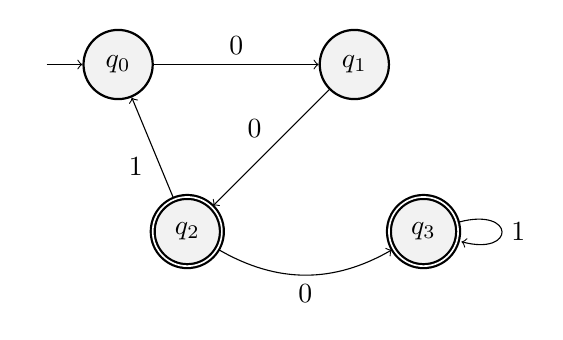
\begin{tikzpicture}
    \node[state, initial] (q0) {$q_0$};
    \node[state, right of = q0] (q1) {$q_1$};
    \node[state, accepting, below left of = q1] (q2) {$q_2$};
    \node[state, accepting, right of = q2] (q3) {$q_3$};
    \draw (q0) edge[above] node{0} (q1)
    (q1) edge[above left] node{0} (q2)
    (q2) edge[below left] node{1} (q0)
    (q2) edge[bend right, below] node{0} (q3)
    (q3) edge[loop right] node{1} (q3);
\end{tikzpicture}

\subsubsection{Criteria for a DFA}

\begin{itemize}
    \item DFAs have exactly one start state.
    \item May have one or more accepting states.
    \item For each state, there must be at most one outgoing transition $\textbf{for each symbol in the alphabet.}$
\end{itemize}

\subsubsection{Language definition with DFAs}

For automaton $M$, the language $L(M)$ consists of all strings $s$ over its alphabet of input symbols statisfying:

\begin{align}
     & q_0 \xrightarrow{\text{s}} * q                                           \\
     & s = q_0,q_1,q_2,...,q_n \text{ for the states: } q_0, q_1, q_2, ..., q_n
\end{align}

If (1) is the case, $s$ is accepted by $M$.
More formally:

\begin{align*}
    L(M) = \{u \mid u \textbf{ is accepted by } M\}
\end{align*}

\subsection{Non-deterministic finite automata}

\subsubsection{What is the difference?}

\begin{itemize}
    \item NDFAs can have multiple outgoing transitions for a given symbol.
    \item NDFAs can have $\epsilon$-transitions, which are transitions that can be taken without consuming an input symbol.
    \item NDFAs can have multiple start states.
    \item NDFAs can have no accepting states.
    \item NDFAs can have multiple accepting states.
\end{itemize}
\subsection{Examples}

Referenced from \url{https://www3.nd.edu/~kogge/courses/cse30151-fa17/Public/other/tikz_tutorial.pdf}.

\subsubsection{DFA 1}

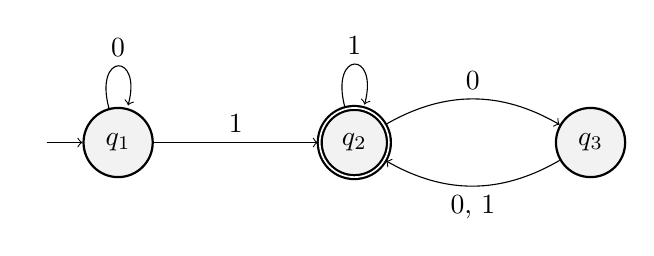
\begin{tikzpicture}
    \node[state, initial] (q1) {$q_1$};
    \node[state, accepting, right of=q1] (q2) {$q_2$};
    \node[state, right of=q2] (q3) {$q_3$};
    \draw (q1) edge[loop above] node{0} (q1)
    (q1) edge[above] node{1} (q2)
    (q2) edge[loop above] node{1} (q2)
    (q2) edge[bend left, above] node{0} (q3)
    (q3) edge[bend left, below] node{0, 1} (q2);
\end{tikzpicture}

\subsubsection{NFA 1}

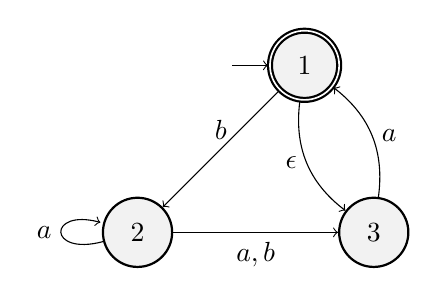
\begin{tikzpicture}
    \node[state, initial, accepting] (1) {$1$};
    \node[state, below left of=1] (2) {$2$};
    \node[state, right of=2] (3) {$3$};
    \draw (1) edge[above] node{$b$} (2)
    (1) edge[below, bend right, left=0.3] node{$\epsilon$} (3)
    (2) edge[loop left] node{$a$} (2)
    (2) edge[below] node{$a, b$} (3)
    (3) edge[above, bend right, right=0.3] node{$a$} (1);
\end{tikzpicture}

\subsubsection{DFA 2}

\begin{figure}
    \centering
    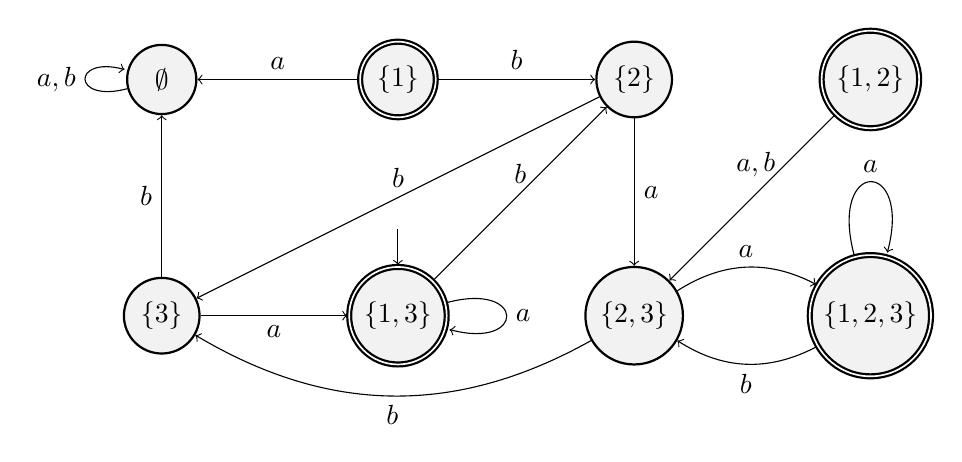
\begin{tikzpicture}
        \node[state] (phi) {$\emptyset$};
        \node[state, accepting, right of=phi] (1) {$\{1\}$};
        \node[state, right of=1] (2) {$\{2\}$};
        \node[state, accepting, right of=2] (12) {$\{1, 2\}$};
        \node[state, below of=phi] (3) {$\{3\}$};
        \node[state, initial, initial where=above, accepting, right of=3] (13) {$\{1, 3\}$};
        \node[state, right of=13] (23) {$\{2, 3\}$};
        \node[state, accepting, right of=23] (123) {$\{1, 2, 3\}$};
        5
        \draw (phi) edge[loop left] node{$a, b$} (phi)
        (1) edge[above] node{$a$} (phi)
        (1) edge[above] node{$b$} (2)
        (2) edge[right] node{$a$} (23)
        (2) edge[above] node{$b$} (3)
        (12) edge[above, pos=.3, left=2pt] node{$a, b$} (23)
        (3) edge[left] node{$b$} (phi)
        (3) edge[below] node{$a$} (13)
        (13) edge[loop right] node{$a$} (13)
        (13) edge[above] node{$b$} (2)
        (23) edge[bend left, above] node{$a$} (123)
        (23) edge[bend left, below] node{$b$} (3)
        (123) edge[loop above] node{$a$} (123)
        (123) edge[bend left, below] node{$b$} (23);
    \end{tikzpicture}
    \caption{DFA} \label{fig:DFA}
\end{figure}


\section{logic}

What does logical thinking in practice look like?

In out daily life we use logic to make decisions, and to make sense of the world around us.
As computers scientists, we have boolean logic machines at our disposal, and we can use them to solve problems.
To take advantage of that, it helps to have a formal and systematic way of thinking about logic.

\subsection{Propositional logic}

The simplest form of formal reasoning is captured by propositional logic.

\subsubsection{Propositional atoms}

Propositional atoms are statements that can be directly evaluated to either true or false.

\begin{itemize}
    \item I have a pen. $ \rightarrow $ True
    \item The sky is blue. $ \rightarrow $ True
    \item Love is a lie. $ \rightarrow $ False
    \item Fire kills. $ \rightarrow $ True
    \item The earth is flat. $ \rightarrow $ False
    \item Peter is openly gay. $ \rightarrow $ True
    \item The moon is made of cheese. $ \rightarrow $ False
    \item My notes will not help my exam. $ \rightarrow $ False
\end{itemize}

\subsubsection{Propositional connective operator symbols}

Here are the table of symbols:

\begin{itemize}
    \item $\neg$ (negation: not)
    \item $\land$ (conjunction: and)
    \item $\lor$ (disjunction: or)
    \item $\implies$ (implication: implies)
    \item $\iff$ (double implication: iff or if and only if)
\end{itemize}

\subsubsection{Truth tables}

Truth tables are a tabular way of representing the truth values of propositional atoms for all possible combinations of truth values.

Here is an example compound proposition:

\begin{align*}
    q \lor r \implies s
\end{align*}

Here is the truth table for the above compound proposition:

\begin{align*}
    \begin{tabular}{|c|c|c|c|}
        \hline
        q & r & s & q $\lor$ r $\implies$ s \\
        \hline
        T & T & T & T                       \\
        \hline
        T & T & F & F                       \\
        \hline
        T & F & T & T                       \\
        \hline
        T & F & F & F                       \\
        \hline
        F & T & T & T                       \\
        \hline
        F & T & F & T                       \\
        \hline
        F & F & T & T                       \\
        \hline
        F & F & F & T                       \\
        \hline
    \end{tabular}
\end{align*}

Logic is cool.

All humans are mortal.
Socrates is a human.
Therefore, Socrates is mortal.
(Example of a Aristotelian syllogism)

\section{Predicate logic}

A predicate is a function that returns a boolean value.

\begin{align*}
    \text{Let } P(x) & = \text{"x is a prime number"} \\
    \text{Let } Q(x) & = \text{"x is a perfect square"}
\end{align*}

\subsection{Quantifiers}

Quantifiers are used to express the extent to which a predicate is true.

\begin{align*}
    \forall x \in \mathbb{N} : P(x) & = \text{"For all x in the set of natural numbers, P(x) is true"} \\
    \exists x \in \mathbb{N} : P(x) & = \text{"There exists an x in the set of natural numbers such that P(x) is true"}
\end{align*}

\subsection{Negation of quantifiers}

\begin{align*}
    \neg \forall x \in \mathbb{N} : P(x) & = \text{"There exists an x in the set of natural numbers such that P(x) is false"} \\
    \neg \exists x \in \mathbb{N} : P(x) & = \text{"For all x in the set of natural numbers, P(x) is false"}
\end{align*}

\subsection{Quantifiers and truth tables}

\begin{align*}
    \begin{tabular}{|c|c|c|c|}
        \hline
        P(x) & Q(x) & $\forall x \in \mathbb{N} : P(x)$ & $\forall x \in \mathbb{N} : Q(x)$ \\
        \hline
        T    & T    & T                                  & T                                \\
        \hline
        T    & F    & F                                  & F                                \\
        \hline
        F    & T    & F                                  & T                                \\
        \hline
        F    & F    & F                                  & F                                \\
        \hline
    \end{tabular}
\end{align*}

\begin{align*}
    \begin{tabular}{|c|c|c|c|}
        \hline
        P(x) & Q(x) & $\exists x \in \mathbb{N} : P(x)$ & $\exists x \in \mathbb{N} : Q(x)$ \\
        \hline
        T    & T    & T                                  & T                                \\
        \hline
        T    & F    & T                                  & F                                \\
        \hline
        F    & T    & T                                  & T                                \\
        \hline
        F    & F    & F                                  & F                                \\
        \hline
    \end{tabular}
\end{align*}

\subsection{Quantifiers and negation}

\begin{align*}
    \neg \forall x \in \mathbb{N} : P(x) & = \exists x \in \mathbb{N} : \neg P(x) \\
    \neg \exists x \in \mathbb{N} : P(x) & = \forall x \in \mathbb{N} : \neg P(x)
\end{align*}




\section{Graphs and trees}

In this section we will be looking at graphs and trees.

\subsection{Graphs}

A graph is a set of vertices and edges (V, E), wjhere:

\begin{itemize}
    \item V is a set of vertices, i.e.: $V = \{v_1, v_2, v_3, ..., v_n\}$
    \item E is a set of edges, i.e.: $E = \{\{v_1, v_2\}, \{v_2, v_3\}, \{v_3, v_4\}, ..., \{v_n, v_1\}\}$
\end{itemize}

NOTICE THAT THE SET OF edges E IS A SET OF SETS, meaning that an edge is an unordered pair of vertices.

Also, there are:

\begin{outline}
    \1 Simple graphs: graphs with no loops or multiple edges
    \1 Multigraphs: graphs with multiple edges between the same two vertices
    \1 Pseudographs: graphs with loops
\end{outline}

\subsection{Directed graphs}

A directed graph is a graph where the edges are directed, i.e.: $(v_1, v_2) \neq (v_2, v_1)$.

\subsubsection{Degree of undirected graphs}

THe degree of a vertex in an undirected graph is the number of edges incident to it, i.e.: $deg(v) = \#\{e \in E \mid v \in e\}$.

\subsubsection{Degree of directed graphs}

The degree of a vertex in a directed graph is the number of edges incident to it, i.e.:
\begin{outline}
    \1 edges that start with v: $deg^+(v) = \#\{e \in E \mid v $ is the first item in the ordered pair $ e\}$.
    \1 edges that end with v: $deg^-(v) = \#\{e \in E \mid v $ is the second item in the ordered pair $ e\}$.
\end{outline}

note that the cardinality of the set of edges incident to a vertex is the sum of the in-degree and out-degree of the vertex, i.e.:

$ \sum_{v \in V} deg^+(v) = \sum_{v \in V} deg^-(v) = \#\{e \in E\} $.

\subsection{isomorphisms}

Two graphs G and H are isomorphic if there exists a bijection $f : V(G) \rightarrow V(H)$ such that:

\begin{align*}
    \forall u, v \in V(G) : \{u, v\} \in E(G) \iff \{f(u), f(v)\} \in E(H)
\end{align*}

Use your fantastic intuition and you will be fine Jim.

\subsection{Paths and Circuits}

A path is a sequence of vertices $v_1, v_2, ..., v_n$ such that $\{v_i, v_{i+1}\} \in E$ for all $i = 1, 2, ..., n-1$.

A circuit is a path that starts and ends at the same vertex.

A path or circuit is simple if all vertices are distinct (does not use the same edge twice).

\subsection{connectedness}

An undirected graph is connected if there is a path between every pair of vertices.

A directed graph is strongly connected if there is a path between every pair of vertices.

A directed graph is weakly connected if the underlying undirected graph is connected.

There might be strongly connected components in a directed graph, where a strongly connected component is a maximal subset of vertices such that every pair of vertices is strongly connected.

\subsection{Eulerian paths and circuits}

Eulerians concern edges, not vertices.

An Eulerian path is a simple path that uses every edge (exactly once, as per previsous definitions of "simple").

An Eulerian circuit is a simple circuit that uses every edge (exactly once, as per previsous definitions of "simple").

Theorem: A connected undirected graph has an Eulerian circuit if and only if every vertex has even degree.

Theorem: A connected undirected graph has an Eulerian path but not an Eulerian circuit if and only if exactly two vertices have odd degree.

SAMPLE GRAPH FOR ILLUSTRATION:

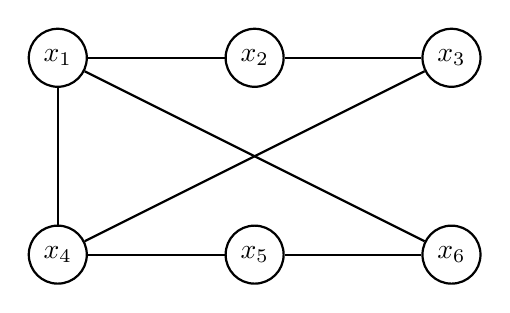
\begin{tikzpicture}[node distance={25mm}, thick, main/.style = {draw, circle}]
    % draw a graph with an Eulerian path but not an Eulerian circuit
    \node[main] (1) {$x_1$};
    \node[main] (2) [right of=1] {$x_2$};
    \node[main] (3) [right of=2] {$x_3$};
    \node[main] (4) [below of=1] {$x_4$};
    \node[main] (5) [right of=4] {$x_5$};
    \node[main] (6) [right of=5] {$x_6$};

    \draw [-] (1) -- (2);
    \draw [-] (2) -- (3);
    \draw [-] (3) -- (4);
    \draw [-] (4) -- (5);
    \draw [-] (5) -- (6);
    \draw [-] (6) -- (1);
    \draw [-] (1) -- (4);
\end{tikzpicture}

\subsection{Hamiltonian paths and circuits}

Hamiltonians concern vertices, not edges.

A Hamiltonian path is a simple path that uses every vertex (exactly once, as per previsous definitions of "simple").

A Hamiltonian circuit is a simple circuit that uses every vertex (exactly once, as per previsous definitions of "simple").


Unlike Eulerians, there is no easy way to determine if a graph has a Hamiltonian path or circuit.

Ayyy lmao.

\subsection{Trees}

A tree is a connected graph with no circuits.

A rooted tree is a tree with a designated root vertex.

The following properties are equivalent for a graph G:

\begin{outline}
    \1 G is a tree.
    \1 There exists exactly one path between any pair of vertices in G.
    \1 G is connected and has exactly n - 1 edges.
    \1 G is connected and either n = 1 and G has no edges,or G <= 2 and removing any edge in G makes the graph unconnected.
    \1 G has no cycles, and adding an edge between any pair of non-adjacent edges v, v creates a cycle containing v and v.

\end{outline}
\subsection{types of traversal}

There are preorder, inorder, and postorder traversals.

\begin{outline}
    \1 Preorder: visit the root, then recursively visit the left and right subtrees.
    \1 Inorder: recursively visit the left subtree, then visit the root, then recursively visit the right subtree.
    \1 Postorder: recursively visit the left and right subtrees, then visit the root.
\end{outline}

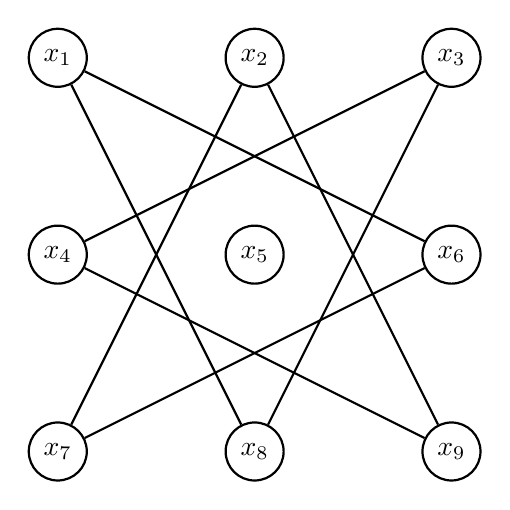
\begin{tikzpicture}[node distance={25mm}, thick, main/.style = {draw, circle}]
    \node[main] (1) {$x_1$};
    \node[main] (2) [right of=1] {$x_2$};
    \node[main] (3) [right of=2] {$x_3$};
    \node[main] (4) [below of=1] {$x_4$};
    \node[main] (5) [right of=4] {$x_5$};
    \node[main] (6) [right of=5] {$x_6$};
    \node[main] (7) [below of=4] {$x_7$};
    \node[main] (8) [right of=7] {$x_8$};
    \node[main] (9) [right of=8] {$x_9$};
    \draw [-] (1) -- (6);
    \draw [-] (1) -- (8);
    \draw [-] (3) -- (4);
    \draw [-] (3) -- (8);
    \draw [-] (4) -- (9);
    \draw [-] (9) -- (2);
    \draw [-] (2) -- (7);
    \draw [-] (7) -- (6);
\end{tikzpicture}

Now onto the 3 $\times$ 4 example.

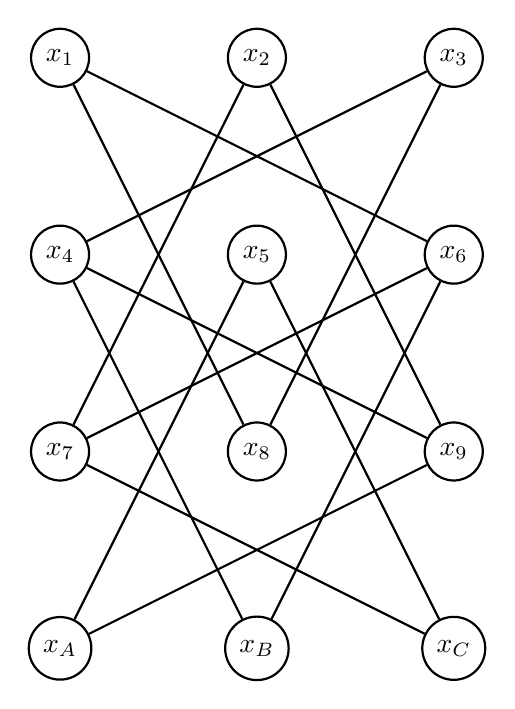
\begin{tikzpicture}[node distance={25mm}, thick, main/.style = {draw, circle}]
    \node[main] (1) {$x_1$};
    \node[main] (2) [right of=1] {$x_2$};
    \node[main] (3) [right of=2] {$x_3$};
    \node[main] (4) [below of=1] {$x_4$};
    \node[main] (5) [right of=4] {$x_5$};
    \node[main] (6) [right of=5] {$x_6$};
    \node[main] (7) [below of=4] {$x_7$};
    \node[main] (8) [right of=7] {$x_8$};
    \node[main] (9) [right of=8] {$x_9$};
    \node[main] (10) [below of=7] {$x_A$};
    \node[main] (11) [right of=10] {$x_B$};
    \node[main] (12) [right of=11] {$x_C$};

    \draw [-] (1) -- (6);
    \draw [-] (1) -- (8);
    \draw [-] (3) -- (4);
    \draw [-] (3) -- (8);
    \draw [-] (4) -- (9);
    \draw [-] (9) -- (2);
    \draw [-] (2) -- (7);
    \draw [-] (7) -- (6);
    \draw [-] (4) -- (11);
    \draw [-] (11) -- (6);
    \draw [-] (12) -- (5);
    \draw [-] (12) -- (7);
    \draw [-] (5) -- (10);
    \draw [-] (10) -- (9);
\end{tikzpicture}

\pagebreak

\section{Proofs}

\begin{itemize}
    \item Definitions are used to create new concepts in terms of existing ones
    \item Axioms are statements that are self evident or assumed to be true
    \item Theorems, Lemmas, Propositions are statements that are shown to be true (via a proof)
    \item Corollary is a property that follows from a Theorem, Lemma or proposition, e.g., as an instance
    \item A proof is a sequence of statements that form an argument using definitions axioms and proof rules
    \item Fanccy ending like "quod erat demonstrandum" is used to indicate the end of a proof.
\end{itemize}


\subsection{Proof methods}

There are four proof methods that we will be using:

\begin{outline}
    \1 Direct proof: Assume the hypothesis and show that the conclusion follows
    \1 Indirect proof (contrapositive, contradiction)
    \2 Contrapositive: Assume the negation of the conclusion and show that the negation of the hypothesis follows
    \2 Contradiction: Assume the hypothesis and the negation of the conclusion and show that a contradiction follows
    % try using latex sub list heirachy below for contrapositive and contradiction
    \1 Existence proofs
    \2 Demonstrate an example that satisfies the hypothesis
    \1 Proof by induction
    \2 Show that the hypothesis holds for the base case
    \2 Show that if the hypothesis holds for an arbitrary case assumed to be true, then it holds for the next case (k + 1)

\end{outline}

\subsection{outline}

Proofs are hard to write, but easy to read.
Proof that the sum of an even number and odd number is odd:

\begin{align*}
    \text{Let } x & = 2k \text{ where } k \in \mathbb{Z}     \\
    \text{Let } y & = 2k + 1 \text{ where } k \in \mathbb{Z} \\
    x + y         & = 2k + 2k + 1                            \\
                  & = 4k + 1                                 \\
                  & = 2(2k) + 1                              \\
                  & = 2k' \text{ where } k' \in \mathbb{Z}   \\
                  & \therefore x + y \text{ is odd}
\end{align*}

\section{Combinatorics and probability}

\subsection{Combinatorics}

\subsubsection{Product rule}

The product rule states that the number of ways to perform a sequence of k tasks, where the first task can be performed in n1 ways, the second task can be performed in n2 ways, and so on, is n1 $\times$ n2 $\times$ ... $\times$ nk.

EXTENDED PRODUCT RULE: The number of ways to perform a sequence of k tasks, where the first task can be performed in n1 ways, the second task can be performed in n2 ways, and so on, and the kth task can be performed in nk ways, is n1 $\times$ n2 $\times$ ... $\times$ nk.

\begin{align*}
    \text{Let } n_1, n_2, n_3, ..., n_k \in \mathbb{N} \\
    \text{The number of ways to perform a sequence of k tasks is:} \\
    n_1 \times n_2 \times n_3 \times ... \times n_k
\end{align*}

\subsubsection{Sum rule}

The sum rule states that the number of ways to perform a task is the sum of the number of ways to perform it in each of several different cases.

\begin{align*}
    \text{Let } n_1, n_2, n_3, ..., n_k \in \mathbb{N} \\
    \text{The number of ways to perform a task is:} \\
    n_1 + n_2 + n_3 + ... + n_k
\end{align*}

\subsubsection{Permutations}

A permutation is an ordered arrangement of objects.

\begin{align*}
    \text{Let } n \in \mathbb{N} \text{ and } k \in \mathbb{N} \text{ where } k \leq n \\
    \text{The number of permutations of n objects taken k at a time is:}                 \\
    P(n, k) = \frac{n!}{(n - k)!}
\end{align*}

\subsubsection{Combinations}

A combination is an unordered selection of objects.

\begin{align*}
    \text{Let } n \in \mathbb{N} \text{ and } k \in \mathbb{N} \text{ where } k \leq n \\
    \text{The number of combinations of n objects taken k at a time is:}                 \\
    C(n, k) = \frac{n!}{k!(n - k)!}
\end{align*}

The symbol $\binom{n}{k}$ is used to denote the number of combinations of n objects taken k at a time.

Sometimes $r$ is used instead of $k$.

\subsection{Probability}

\subsubsection{Sample space}

The sample space is the set of all possible outcomes of an experiment.

\subsubsection{Event}

An event is a subset of the sample space.

\subsubsection{Probability}

The probability of an event is the number of outcomes in the event divided by the number of outcomes in the sample space.

\begin{align*}
    \text{Let } S \text{ be the sample space and } E \subseteq S \text{ be an event} \\
    P(E) = \frac{\#E}{\#S}
\end{align*}

\subsubsection{Probability axioms}

\begin{outline}
    \1 $0 \leq P(E) \leq 1$
    \1 $P(S) = 1$
    \1 If $E_1, E_2, E_3, ...$ are disjoint events, then $P(E_1 \cup E_2 \cup E_3 \cup ...) = P(E_1) + P(E_2) + P(E_3) + ...$
\end{outline}

\subsubsection{Probability rules}

\begin{outline}
    \1 $P(E^c) = 1 - P(E)$
    \1 $P(E \cup F) = P(E) + P(F) - P(E \cap F)$
    \1 $P(E \cup F \cup G) = P(E) + P(F) + P(G) - P(E \cap F) - P(E \cap G) - P(F \cap G) + P(E \cap F \cap G)$
\end{outline}

\subsubsection{Conditional probability}

The conditional probability of an event E given an event F is the probability of E given that F has occurred.

\begin{align*}
    \text{Let } E, F \text{ be events such that } P(F) > 0 \\
    P(E \mid F) = \frac{P(E \cap F)}{P(F)}
\end{align*}

\subsubsection{Independence}

Two events E and F are independent if $P(E \cap F) = P(E)P(F)$.

\subsubsection{Bayes' theorem}

\begin{align*}
    \text{Let } E, F \text{ be events such that } P(E) > 0 \text{ and } P(F) > 0 \\
    P(E \mid F) = \frac{P(F \mid E)P(E)}{P(F)}
\end{align*}

\subsubsection{Random variables}

A random variable is a function that assigns a real number to each outcome in the sample space.

\subsubsection{Probability distribution}

The probability distribution of a random variable X is the function that assigns a probability to each real number x.

\begin{align*}
    \text{Let } X \text{ be a random variable} \\
    p(x) = P(X = x)
\end{align*}

\subsubsection{Expected value}

The expected value of a random variable X is the sum of the product of each possible value of X and its probability.

\begin{align*}
    \text{Let } X \text{ be a random variable} \\
    E(X) = \sum_{x \in X(S)} x \cdot p(x)
\end{align*}

\subsubsection{Variance}

The variance of a random variable X is the expected value of the squared difference between X and its expected value.

\begin{align*}
    \text{Let } X \text{ be a random variable} \\
    \sigma_X = 
\end{align*}

\subsubsection{Standard deviation}

The standard deviation of a random variable X is the square root of its variance.

here is the formula for standard deviation:

\begin{align*}
    \text{Standard deviation} = \sqrt{\text{Variance}} \\
    \text{Or more formally:} \\
    \sigma = \sqrt{Var(X)}
\end{align*}

\subsubsection{Bernoulli trials}

A Bernoulli trial is an experiment with two possible outcomes: success or failure, such that:

\begin{outline}
    \1 The probability of success is p
    \1 The probability of failure is 1 - p
    \1 The trials are independent
\end{outline}

\subsubsection{Binomial distribution}

The binomial distribution is the probability distribution of the number of successes in a sequence of n independent Bernoulli trials.

\begin{align*}
    \text{Let } X \text{ be a random variable} \\
    p(x) = P(X = x) = \binom{n}{x} p^x (1 - p)^{n - x}
\end{align*}

\section{Previous mistakes list}

\begin{outline}
    \1 A group of animals consists of m cats and m dogs. How many ways are there to arrange the animals in a line if cats must alternate with dogs?
        \2 $2(m!)^2$ because: The line can either start with a cat or with a dog, giving two possibilities. \\
    Once this is fixed, the cats can be permuted arbitrary, giving $ m! $ possibilities, and the the dogs can be permuted arbitrary, giving $ m! $ possibilities as well. Overall, there are $2(m!)^2$ possibilities.
    \1 Below, you will see some specific types of logical statements. \\
    Sort them according to the following order: \\
    -- rank top (number 1) those than are most often necessarily true \\
    -- rank bottom (number 4) those than are most often necessarily false \\
    -- in between cases a and b, rank bottom those that are necessarily false more often.\\
    \2 Contradiction: always false \\
    Tautology: always true \\
    Contingent: This is sometimes true, sometimes false. Since it is necessarily at least once false, then it ranks lower than satisfiable. \\
    Satisfiable: At least once trues. This can still mean always true and therefore never false. \\
    \1 There can be a language corresponding to regular expression $ \emptyset $.
\end{outline}
\end{document}
